% !TEX program = latexmk
% !TEX options = -xelatex --shell-escape -synctex=1 -interaction=nonstopmode -halt-on-error -file-line-error -f "%DOC%"

\documentclass[preview,tikz,dvipsnames, border=12pt,convert={density=600, png}]{standalone}

% Fonts
\usepackage{bold-extra}

% Math, Vectors, Magnitude
\usepackage{amssymb,amsfonts,amsmath}
\usepackage{bm}
\newcommand{\vect}[1]{\mathbf{#1}}

% Color
\definecolor{UbuntuOrange}{HTML}{E95420}
\definecolor{UbuntuPurple}{HTML}{77216F}
\definecolor{ROSBlue}{HTML}{22314E}
\definecolor{PythonBlue}{HTML}{306998}
\definecolor{PythonYellow}{HTML}{FFD43B}
\definecolor{PythonOrange}{HTML}{FFB13B}
\definecolor{GazeboOrange}{HTML}{F58113}
\definecolor{GazeboWhite}{HTML}{FFFFFF}
\definecolor{IgnitionLightOrange}{HTML}{E5B533}
\definecolor{IgnitionDarkOrange}{HTML}{DE6921}


% Figures
\usepackage{graphicx}

% TIKZ
\usetikzlibrary{quotes,angles,calc,shapes,arrows.meta,positioning, decorations.markings, backgrounds}

\tikzset{
  event/.style = {circle, fill, minimum size=1, line width=.1pt},
  timeline/.style = {draw, thick,  shorten <=10pt,shorten >=10pt},
  % pics/ubuntu/.style args={#1/#2} {
  %   code={
  %     \node[event=1pt, shading=axis, left color=UbuntuPurple, right color = UbuntuOrange, shading angle = 135] (#2) at (0,0){};
  %     \node[below=0.1 of bionic]{\texttt{Bionic}};
  %   }
  % },
  % event/.default = 10pt,
  % block/.style = {draw, rectangle, minimum height=2em, minimum width=3em},
  % sum/.style = {draw, circle, node distance=1cm, minimum size = 0.5cm},
  arrow/.style={thick, ->},
  line/.style={thick, -},
  white background/.style={
        show background rectangle,
        tight background,
        background rectangle/.style={
            fill=white
        }
    }
}

\newcommand{\distrubuntu}[2]{% name, year
  \def\year{#2}
  \pgfmathsetmacro\x{2*(\year-2016)};
  \node[event=1.5pt, shading=axis, left color=UbuntuPurple, right color = UbuntuOrange, shading angle=135] (#1) at (\x,-1){};
  \node[below=0.1 of #1]{\textcolor{UbuntuPurple}{\texttt{#1}}};
}

\newcommand{\distrros}[2]{% name, year
  \def\year{#2}
  \pgfmathsetmacro\x{2*(\year-2016)};
  \node[event=1.5pt, fill=ROSBlue] (#1) at (\x,-2.5){};
  \node[below=0.1 of #1]{\textcolor{ROSBlue}{\texttt{#1}}};
}

\newcommand{\distrrostwo}[2]{% name, year
  \def\year{#2}
  \pgfmathsetmacro\x{2*(\year-2016)};
  \node[event=1.5pt, fill=ROSBlue] (#1) at (\x,-4){};
  \node[below=0.1 of #1]{\textcolor{ROSBlue}{\texttt{#1}}};
}

\newcommand{\pythonversion}[2]{% name, year
  \def\year{#2}
  \pgfmathsetmacro\x{2*(\year-2016)};
  \node[event=1.5pt, shading=axis, left color=PythonBlue, right color=PythonYellow, shading angle=45] (Python#2) at (\x,-5.5){};
  \node[below=0.1 of Python#2]{\textbf{#1}};
}

\newcommand{\gazeboversion}[2]{% name, year
  \def\year{#2}
  \pgfmathsetmacro\x{2*(\year-2016)};
  \node[event=1.5pt, shading=axis, left color=GazeboOrange, right color=GazeboWhite, shading angle=10] (Gazebo#2) at (\x,-5.5){};
  \node[below=0.1 of Gazebo#2]{\textbf{#1}};
}

\newcommand{\ignitionversion}[2]{% name, year
  \def\year{#2}
  \pgfmathsetmacro\x{2*(\year-2016)};
  \node[event=1.5pt, shading=axis, left color=IgnitionLightOrange, right color=IgnitionDarkOrange, shading angle=45] (Ignition#2) at (\x,-7){};
  \node[below=0.1 of Ignition#2]{\textbf{#1}};
}

\newcommand{\rosdistro}[1]{\textcolor{ROSBlue}{\texttt{#1}}}

\def\figScale{1}
\def\xLogo{-2}

\begin{document}

\begin{tikzpicture}[
    scale=\figScale,
    white background,
  ]
  \node(year) at (\xLogo, 0) {\textbf{Year}};
  \foreach \x in {0,2,...,16}
  \pgfmathtruncatemacro{\year}{\x/2+2016}
  \node (\year) at (\x,0) {\textbf{\year}};

  % ubuntu
  \node[inner sep=0pt] (ubuntu) at (\xLogo,-1) {
    
\includegraphics[height=1cm]{assets/Ubuntu.png}
  };
  \distrubuntu{xenial}{2016};
  \distrubuntu{bionic}{2018};
  \distrubuntu{focal}{2020};
  \distrubuntu{jammy}{2022};
  \distrubuntu{noble}{2024};
  \draw[timeline, UbuntuPurple] (xenial) -- (bionic);
  \draw[timeline, UbuntuPurple] (bionic) -- (focal);
  \draw[timeline, UbuntuPurple] (focal) -- (jammy);
  \draw[timeline, UbuntuPurple] (jammy) -- (noble);

  % ros
  \node[inner sep=0pt] (ros) at (\xLogo,-2.5) {
    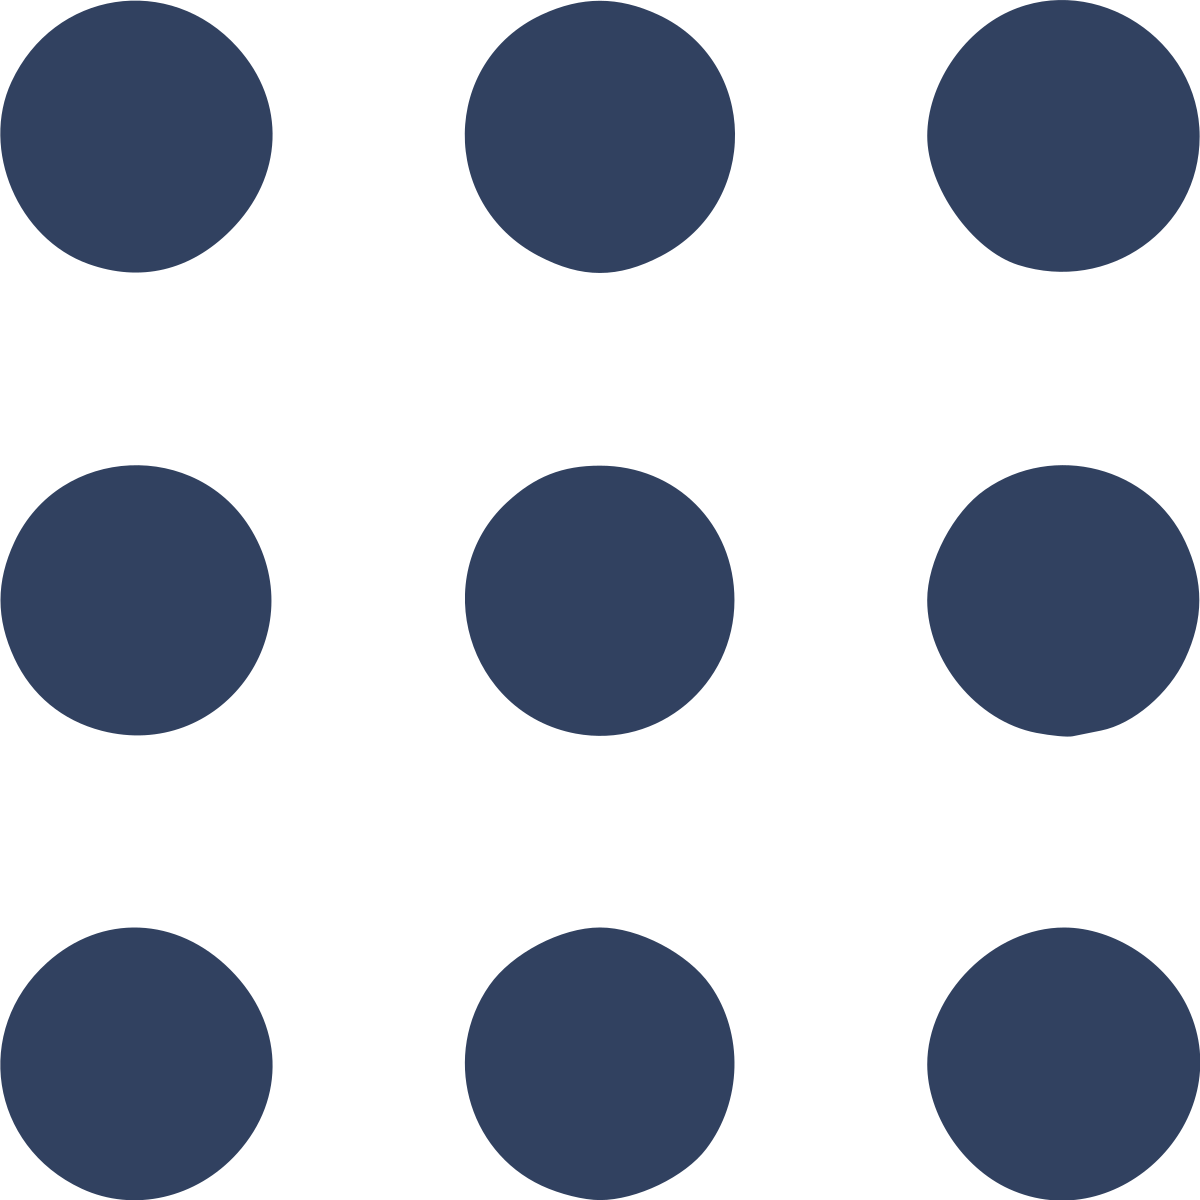
\includegraphics[height=0.75cm]{assets/ros.png}
  };
  \distrros{kinetic}{2016}
  \distrros{lunar}{2017}
  \distrros{melodic}{2018}
  \distrros{noetic}{2020}
  \draw[timeline, ROSBlue] (kinetic) -- (lunar);
  \draw[timeline, ROSBlue] (lunar) -- (melodic);
  \draw[timeline, ROSBlue] (melodic) -- (noetic);

  \node[inner sep=0pt] (ros2) at (\xLogo,-4) {
    
\includegraphics[width=0.75cm]{assets/ros2.png}
  };

  \distrrostwo{foxy}{2020}
  \distrrostwo{galactic}{2021}
  \distrrostwo{humble}{2022}
  \distrrostwo{iron}{2023}
  \distrrostwo{jazzy}{2024}
  \draw[timeline, ROSBlue] (foxy) -- (galactic);
  \draw[timeline, ROSBlue] (galactic) -- (humble);
  \draw[timeline, ROSBlue] (humble) -- (iron);
  \draw[timeline, ROSBlue] (iron) -- (jazzy);

  \begin{scope}[opacity=0.75]
    \def\eloquentYear{2019}
    \pgfmathsetmacro\x{2*(\eloquentYear-2016)};
    \node[event=1.5pt, fill=ROSBlue] (eloquent) at (\x,-4){};
    \node[below=0.1 of eloquent,align=center]{\rosdistro{dashing}\\\rosdistro{eloquent}};
    \draw[timeline, ROSBlue] (eloquent) -- (foxy);
  \end{scope}

  \begin{scope}[opacity=0.75]
    \def\ardentYear{2018}
    \pgfmathsetmacro\x{2*(\ardentYear-2016)};
    \node[event=1.5pt, fill=ROSBlue] (ardent) at (\x,-4){};
    \node[below=0.1 of ardent,align=center]{\rosdistro{ardent}-\\\rosdistro{crystal}};
    \draw[timeline, ROSBlue] (ardent) -- (eloquent);
  \end{scope}


  % % Python
  % \node[inner sep=0pt] (python) at (\xLogo,-5.5) {
  %   
\includegraphics[width=0.75cm]{python.png}
  % };
  % \pythonversion{\textcolor{PythonOrange}{2.7}/\textcolor{PythonBlue}{3.5}}{2016}
  % \pythonversion{\textcolor{PythonOrange}{2.7}/\textcolor{PythonBlue}{3.6}}{2018}
  % \pythonversion{\textcolor{PythonBlue}{3.8}}{2020}
  % \pythonversion{\textcolor{PythonBlue}{3.10}}{2022}
  % \pythonversion{\textcolor{PythonBlue}{3.12}}{2024}
  % \draw[timeline, PythonBlue] (Python2016) -- (Python2018);
  % \draw[timeline, PythonBlue] (Python2018) -- (Python2020);
  % \draw[timeline, PythonBlue] (Python2020) -- (Python2022);
  % \draw[timeline, PythonBlue] (Python2022) -- (Python2024);
  
  % Gazebo
  \node[inner sep=0pt] (gazebo) at (\xLogo,-5.5) {
    
\includegraphics[width=0.75cm]{assets/Gazebo.png}
  };
  \gazeboversion{\textcolor{GazeboOrange}{7.x}}{2016}
  \gazeboversion{\textcolor{GazeboOrange}{9.x}}{2018}
  \gazeboversion{\textcolor{GazeboOrange}{11.x}}{2020}
  \gazeboversion{}{2023}
  \draw[timeline, GazeboOrange] (Gazebo2016) -- (Gazebo2018);
  \draw[timeline, GazeboOrange] (Gazebo2018) -- (Gazebo2020);
  \draw[timeline, GazeboOrange] (Gazebo2020) -- (Gazebo2023);
  
  % Ignition
  \node[inner sep=0pt] (ignition) at (\xLogo,-7) {
    
\includegraphics[width=0.75cm]{assets/Ignition.png}
  };
  \ignitionversion{\textcolor{IgnitionDarkOrange}{citadel}}{2020}
  \ignitionversion{\textcolor{IgnitionDarkOrange}{edifice}}{2021}
  \ignitionversion{\textcolor{IgnitionDarkOrange}{fortress}}{2022}
  \ignitionversion{\textcolor{IgnitionDarkOrange}{harmonic}}{2024}
  \draw[timeline, IgnitionLightOrange] (Ignition2020) -- (Ignition2021);
  \draw[timeline, IgnitionLightOrange] (Ignition2021) -- (Ignition2022);
  \draw[timeline, IgnitionLightOrange] (Ignition2022) -- (Ignition2024);

\end{tikzpicture}

\end{document}